\documentclass{article}
\usepackage{tikz}
\usepackage{geometry}
\usepackage{amsmath}
\geometry{margin=1in}

\title{Unified Implementation Plan for Autonomous CNC Toolpath System}
\author{M365 Copilot}
\date{\today}

\begin{document}
\maketitle

\section{Included Source Prompts}
\subsection{Toolpath Prompt}
\textit{You are a software+mechanical engineer tasked with generating a toolpath generation software... tool must enter from outside the face.}

\subsection{Feeds and Speeds Context}
\textit{You are selecting feeds and speeds based on material, tool, and operation with shop-floor adjustments.}

\subsection{Factory Simulation Prompt}
\textit{You are developing a simulation of an autonomous factory with multiple CNC machines, toolpaths, scheduling, and optimization policies.}

\section{System Architecture}

\begin{center}
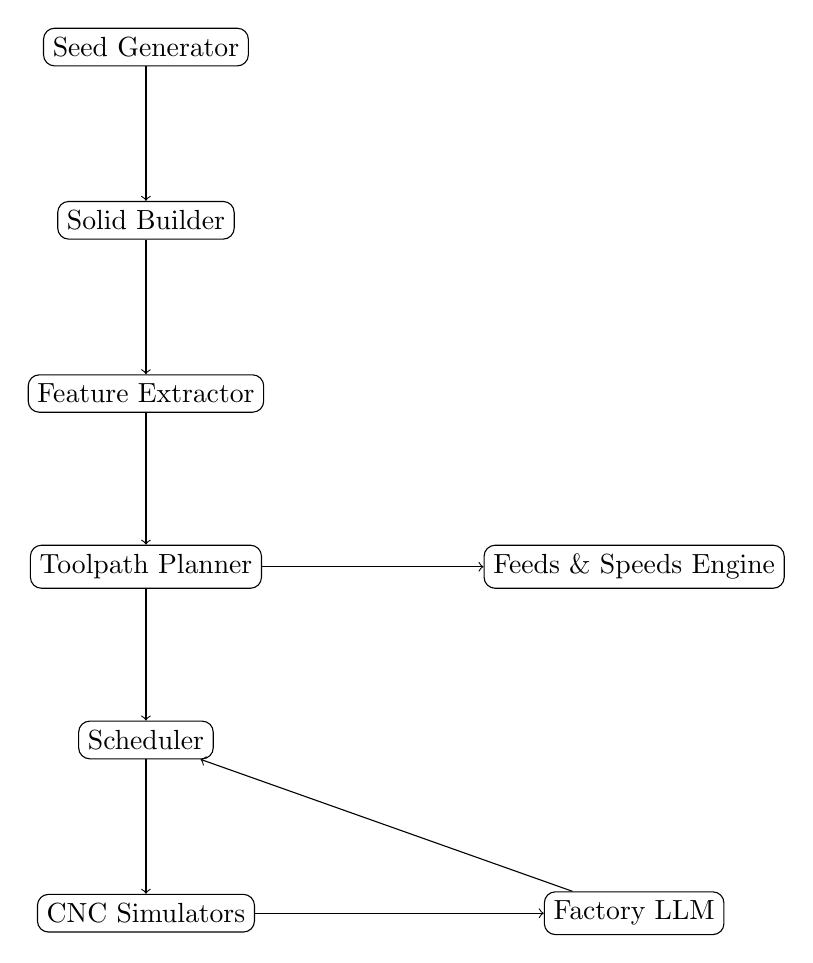
\begin{tikzpicture}[node distance=2.2cm, every node/.style={draw, rectangle, rounded corners}]

\node (seed) {Seed Generator};
\node (solid) [below of=seed] {Solid Builder};
\node (features) [below of=solid] {Feature Extractor};
\node (planner) [below of=features] {Toolpath Planner};
\node (fs) [right of=planner, xshift=4cm] {Feeds \& Speeds Engine};
\node (scheduler) [below of=planner] {Scheduler};
\node (machines) [below of=scheduler] {CNC Simulators};
\node (factory) [right of=machines, xshift=4cm] {Factory LLM};

\draw[->] (seed) -- (solid);
\draw[->] (solid) -- (features);
\draw[->] (features) -- (planner);
\draw[->] (planner) -- (scheduler);
\draw[->] (scheduler) -- (machines);
\draw[->] (planner) -- (fs);
\draw[->] (machines) -- (factory);
\draw[->] (factory) -- (scheduler);

\end{tikzpicture}
\end{center}

\section{Implementation Modules}

\subsection{1. Solid Builder}
- Generate 1--4 cuboids (axis-aligned)
- Add pockets and holes
- Output: face list with wall/cliff metadata

\subsection{2. Feature Extractor}
- Identify top faces P$_i$
- Label edges: Wall / Cliff / Level

\subsection{3. Toolpath Planner}
Core algorithm:\\
- Classify edges (wall, cliff) \cite{toolpath} \\
- Compute safe region $S_i = P_i \ominus B_{blocked}$ \cite{toolpath} \\
- Generate raster paths
- Ensure entry from safe edge

\subsection{4. Feeds \& Speeds Engine}
- Compute RPM from cutting speed \cite{feeds} \\
- Compute feed: $F = N Z f_z$ \cite{feeds}
- Adjust based on chatter, rigidity

\subsection{5. Drilling \& Entry Module}
- Peck drilling rules (0.25D--1D) \cite{feeds}
- Entry selection (plunge, ramp, helix)

\subsection{6. Scheduler}
- Assign parts to machines
- Optimize based on policy:
\begin{itemize}
\item Min time
\item Max tool life
\item Min cost
\item Best finish
\end{itemize}

\subsection{7. CNC Simulator}
- Execute G-code
- Track:
\begin{itemize}
\item Tool wear
\item Time
\item Errors
\end{itemize}

\section{Algorithm Pipeline}
\begin{verbatim}
seed -> build geometry -> extract features
-> generate toolpath -> assign feeds/speeds
-> schedule -> simulate -> feedback
\end{verbatim}

\section{Key Data Structures}
\begin{itemize}
\item Face: polygon + height + edges
\item Tool: diameter, life, cost
\item Machine: queue, tool crib
\item Feature: pocket, hole, face
\end{itemize}

\section{Weaknesses and Missing Information}

\subsection{Geometry Limitations}
- Only cuboids supported
- No curved surfaces or rotations

\subsection{Toolpath Gaps}
- No cutter deflection modeling
- No corner smoothing/blending

\subsection{Physics Gaps}
- No cutting force model
- No power/torque constraints

\subsection{Feeds \& Speeds Limitations}
- Empirical only (no adaptive control)
- Missing tool coating effects

\subsection{Simulation Gaps}
- Tool crib not fully implemented
- Error handling incomplete
- Multi-machine coordination unclear

\subsection{Optimization Gaps}
- Multi-objective optimization not formalized
- No global optimization across features

\subsection{Software Gaps}
- Dependency on outdated OCC environment
- No API contract between modules

\section{Recommended Improvements}
\begin{itemize}
\item Add force and power models
\item Implement adaptive feed control
\item Extend geometry kernel
\item Formalize API between modules
\item Add unit tests and benchmarking
\end{itemize}

\section{Hierarchical Error-Aware Multi-Agent Control System}

\subsection{Overview}
To address the current gap in error handling and multi-machine coordination, we introduce a hierarchical, LLM-driven control architecture enabling real-time anomaly interpretation, safe intervention, and coordinated mitigation across CNC agents and the factory system.

This system augments the existing CNC simulator and factory-level orchestration with:
\begin{itemize}
    \item Interactive human-in-the-loop input
    \item Structured prompt-to-context transformation
    \item Local (CNC) and global (Factory) agent reasoning
    \item Safety-aware execution and escalation
\end{itemize}

\subsection{System Architecture}

The extended control loop is defined as:

\begin{center}
\texttt{User Input $\rightarrow$ Context Transformer $\rightarrow$ CNC Agent LLM $\rightarrow$ Safety Evaluator $\rightarrow$ (Escalation) $\rightarrow$ Factory Agent LLM $\rightarrow$ Mitigation Execution}
\end{center}

\subsection{CNC Agent Extensions}

\subsubsection{Simulation Dashboard}
Each CNC simulator is extended with:
\begin{itemize}
    \item Real-time toolpath and material removal visualization
    \item Machine telemetry (feed, RPM, load, tool state)
    \item \textbf{Interactive dialog box} for prompt input
\end{itemize}

The dialog box allows users to:
\begin{itemize}
    \item Report anomalies (e.g., chatter, collision risk)
    \item Inject scenario-based conditions
    \item Directly interact with the simulation
\end{itemize}

\subsubsection{Prompt-to-Context Transformation}

Natural language prompts are transformed into structured representations:

\begin{verbatim}
{
  event_type: anomaly,
  category: vibration,
  severity: unknown,
  location: boundary_region,
  machine_state: {...}
}
\end{verbatim}

This ensures that LLM reasoning is grounded in machine state rather than raw text.

\subsubsection{CNC Agent LLM}

The CNC agent LLM:
\begin{itemize}
    \item Interprets structured context
    \item Proposes corrective actions
\end{itemize}

Example output:
\begin{verbatim}
{
  action: reduce_feed,
  parameters: {factor: 0.8},
  risk_level: moderate
}
\end{verbatim}

\subsubsection{Safety Evaluator}

All LLM outputs are classified into:

\begin{itemize}
    \item \textbf{Safe}: minor parameter adjustments
    \item \textbf{Risky}: significant modifications requiring monitoring
    \item \textbf{Catastrophic}: unsafe operations (e.g., collision risk)
\end{itemize}

\subsubsection{Catastrophic Response Handling}

If a catastrophic response is detected:
\begin{itemize}
    \item Immediately pause machine execution
    \item Capture machine state (tool position, G-code index, telemetry)
    \item Escalate context to the factory agent
\end{itemize}

\subsection{Factory Agent System}

\subsubsection{Factory Dashboard}

A global interface providing:
\begin{itemize}
    \item Multi-machine state visualization
    \item Production KPIs
    \item Interactive dialog interface
\end{itemize}

Supported commands include:
\begin{itemize}
    \item Query machine state
    \item Stop production
    \item Modify scheduling and tooling policies
\end{itemize}

\subsubsection{Factory Agent LLM}

The factory agent:
\begin{itemize}
    \item Performs system-level diagnosis
    \item Aggregates machine-level context
    \item Generates mitigation strategies
\end{itemize}

Example mitigation output:
\begin{verbatim}
{
  diagnosis: tool chatter near thin wall,
  actions: [
    {target: cnc_agent_5, command: reduce_feed, factor: 0.6},
    {target: scheduler, command: adjust_policy}
  ]
}
\end{verbatim}

\subsection{Multi-Agent Coordination}

Agents communicate using structured messages:

\begin{verbatim}
{
  sender: factory_agent,
  receiver: cnc_agent_5,
  type: mitigation_command,
  payload: {...}
}
\end{verbatim}

Coordination patterns include:
\begin{itemize}
    \item Local correction (single CNC agent)
    \item Global policy update (scheduler or feeds/speeds)
    \item Multi-machine coordination
\end{itemize}

\subsection{Integrated Execution Loop}

The original pipeline:
\begin{center}
\texttt{simulate $\rightarrow$ feedback}
\end{center}

is extended to:
\begin{center}
\texttt{simulate $\rightarrow$ prompt $\rightarrow$ transform $\rightarrow$ CNC LLM $\rightarrow$ safety check $\rightarrow$ (escalate) $\rightarrow$ factory LLM $\rightarrow$ mitigate $\rightarrow$ resume}
\end{center}

\subsection{Design Principles}

\begin{itemize}
    \item \textbf{Separation of Concerns}: CNC agent (local) vs Factory agent (global)
    \item \textbf{Structured Context}: no raw prompt reasoning
    \item \textbf{Safety First}: hard stop before unsafe execution
    \item \textbf{Human-in-the-Loop}: dialog interfaces enable supervision
\end{itemize}

\subsection{Impact on Existing System}

This extension directly addresses gaps identified in Section 6:
\begin{itemize}
    \item Completes error handling architecture
    \item Enables multi-machine coordination
    \item Provides a foundation for adaptive and autonomous control
\end{itemize}

\section{Conclusion}
This unified plan integrates geometry generation, toolpath planning, machining parameters, and factory-level scheduling into a single modular system suitable for implementation.

\end{document}
